\chapter[Throwing polarised light on some mathematics: Mysore, November 8-9 2012]{Throwing polarised light on some mathematics: Mysore, November 8-9 2012}\label{chap26}

%\Authorline{N.G.Deshpande// Professor of Physics, University of Oregon}

\begin{center}
\textbf{Rajaram Nityananda}
%\textbf{\textit{Professor of Physics (retd.), Bangalore University}}
\end{center}

The physics of plane, perfectly monochromatic wave is simply summarised
in the electric field vector whose two orthogonal components are given by
$E_1 = a_1 \cos(wt - \phi_1)$; $E_2 = a_2 \cos(wt - \phi_2)$ or using basis vectors $\hat{e}_1$ and $\hat{e}_2$
\begin{gather*}
\overrightarrow{E} = Re (a_1 e^{i \phi_1 } \hat{e}_1 + a_2 e^{i\phi_2} \hat{e}_2 ) e^{-i\omega t} \\
\equiv Re \overrightarrow{\varepsilon} e^{-i\omega t}
\end{gather*}

The coefficient of the harmonic time dependence $e^{-i \omega t}$ is the complex two dimensional vector
$\overrightarrow{\varepsilon} = z_1 \hat{e}_1 + z_2 \hat{e}_2$ where $z_1$, $z_2$ encode the amplitude and the phase of each of
the components $- z_1 = a_1 e^{i \phi_1}$, $z_2 = a_2 e^{i\phi_2}$. Mathematician's call such a space
$\mathbb{C}^2$ (for two dimensional complex vector space). The operation which comes
naturally with such a space also have natural physical counter parts.
\begin{itemize}
\item[a)] Superposition $\overrightarrow{\varepsilon}_1 + \overrightarrow{\varepsilon}_2$ is realised as interference e.g using a half silvered
mirror as in the Michelson interferometer $\overrightarrow{\varepsilon}$ is proportional to $\overrightarrow{\varepsilon}_1 + \overrightarrow{\varepsilon}_2$ (ideally
$\dfrac{1}{\sqrt{2}} (\overrightarrow{\varepsilon}_1 + \overrightarrow{\varepsilon}_2)$)
\begin{figure}[H]
\centering
\includegraphics[scale=0.1]{src/images/chap26/1.eps}
\end{figure}

\item[b)] Scalar multiplication $\overrightarrow{\varepsilon}' \to re^{i\theta} \overrightarrow{\varepsilon}$ for $r < 1$ this is the attenuator (dark
glass!) which cuts down the amplitude by $r$, $\theta$ is a phase retardation (parallel slab of transparent glass), $r > 1$, amplification also became possible after lasers


\item[c)] Norm in a complex vector space is the counterpart of ``squared length" in
our familiar vectors. The intensity of our wave is proportional to $a_1^2 + a_2^2$ after
averaging over a period. This can be written as $I = | z_1 |^2 + | z_2 |^2$ $\equiv z^{\ast}_1 z_1 + z^{\ast}_2 z_2$ $\equiv \overrightarrow{\varepsilon}^{\ast} \cdot \overrightarrow{\varepsilon}$ (notice that $\ast$ in over the first $\overrightarrow{\varepsilon}$, it's important)

\item[d)] A typical experiment is to combine two different beams $\overrightarrow{\varepsilon}$ and $\overrightarrow{\varepsilon}'$ apply a phase
shift $\psi$ to $\overrightarrow{\varepsilon}'$, and measure the total intensity, using (a), (b) and (c) above, this
gives:
\begin{align*}
I_{tot} & = (\overrightarrow{\varepsilon}^{\ast} + \overrightarrow{\varepsilon}'^{\ast} e^{-i\psi})  \cdot (\overrightarrow{\varepsilon} + \overrightarrow{\varepsilon}' e^{i\psi})\\
& = \overrightarrow{\varepsilon}^{\ast} \cdot \overrightarrow{\varepsilon} + \overrightarrow{\varepsilon}'^{\ast}  \cdot \overrightarrow{\varepsilon}' + (\overrightarrow{\varepsilon}^{\ast} \cdot \overrightarrow{\varepsilon}' e^{i\psi}  + \text{ its complex conjugate}).
\end{align*}

The first two terms are just the intensity of $\overrightarrow{\varepsilon}$ and $\overrightarrow{\varepsilon}'$ by themselves. Our focus will be on the interference term which can be written out in full as $Re(\overrightarrow{\varepsilon}^{\ast}  \cdot \overrightarrow{\varepsilon}') \cos \psi + \Iim (\overrightarrow{\varepsilon}^{\ast} \cdot \overrightarrow{\varepsilon}') \sin \psi$
Since $\psi$ can be varied, both the real and imaginary parts of ($\overrightarrow{\varepsilon}^{\ast} \cdot \overrightarrow{\varepsilon}'$) can be
measured. Mathematically, this is the ``inner product", and the norm is just
the inner product of a vector with itself. We can also write the interference
term as $\| \overrightarrow{\varepsilon}^{\ast}  \cdot \overrightarrow{\varepsilon}'\| e^{i\phi_{EE'}} \cdot e^{i\phi}$ where $\phi_{\varepsilon \varepsilon'}$ is the phase of our inner product and $\psi$ our added phase in the $\varepsilon'$ beam. The intensity of this term now reads
$| \overrightarrow{\varepsilon}^{\ast} \cdot \overrightarrow{\varepsilon}| \cos (\phi_{EE'} + \psi)$ and is a maximum when $\psi = -\phi_{EE]}$. Pancharatnam
used this criterion to define the phase retardation of $\overrightarrow{\varepsilon}'$ with respect to $\varepsilon$, when
they are in different states of polarization. Namely, since retardation of $-\phi_{\varepsilon \varepsilon}'$ 
given to $\varepsilon'$ maximises the intensity, i.e, brings them `in phase', it's logical to
think of $\phi_{\varepsilon \varepsilon'}$ in this way. We returned to this later!

\item[e)] The definition fails in one case, when the inner product is zero. The simplest
example would be $\varepsilon = \alpha \hat{e}_1$, $\varepsilon = \alpha' \hat{e}_2$. This is one of the ``Fresnel Argo laws" for
interference of polarized light - two linearly polarized beams in perpendicular
directions do not interfere. More correctly, we should say that as we vary the
relative phase, the intensity does not change. We can see that any two beams
satisfying $a^{\ast} \cdot b = 0$ will show this non interference in intensity - they are called
orthogonal.

\item[f)] So far, our vectors have been expressed in terms of $\hat{e}_1$ and $\hat{e}_2$, two unit intensity
linearly polarized beams. A vector space like $\mathbb{C}^2$ comes with the freedom to
change the basis. For example, define $\hat{e}_R = \dfrac{\hat{e}_1 + i \hat{e}_2}{\sqrt{2}}$


\end{itemize}

%%%

\end{document}


~ε ≡ Z 1 ê 1 +Z 2 ê 2 ≡ Z R ê R +Z L ê L where the amplitudes of the R and L beams
are
+iZ 2
−iZ 2
Z R = Z 1 √
; Z L = Z 1 √
2
2
ê R and ê L are just one example of an orthonormal basis pair but have a simple
physical meaning. ê R is an equal superposition of beams along x and y, with
y retarded by a phase lag of π/2 (hence the i in front of ê 2 ). In such a beam,
the tip of the electric vector describes a circle, (E x = a cos wt, E y = a sin wt)
traversed counter clockwise when facing the source. This is called ‘ right circu-
larly polarized’ or RCP light. Retarding it in phase moves the vector clockwise.
LCP has the the opposite sense since E y leads E x by π/2. RCP carries angular
momentum along the direction of propagation and LCP opposite to it (like off
spin and leg spin in cricket!)





